\chapter{Restarts, ensembles and calibration}\label{uch:restarts}
This chapter covers what you do with a working model: start it well, split or continue long runs, run ensembles and
calibrate. Workshop~5 practises restarts, ensembles and particle tracking; Workshop~6 calibration with Ostrich.

\section{Spin-up}
\paragraph{How long a spin-up do I need?} Start from a steady state with the long-term mean recharge
(\cmd{:GWInitialization STEADY\_STATE r}, Section~\ref{sec:ustart}). Then check that \emph{storage release} in
\cmd{GWBudget.csv} averages near zero over the first years. Large, slow aquifers may need decades.

\section{Restarts (hotstart)}\label{sec:urestart}
At the end of a run Raven writes \cmd{solution.rvc}. Besides Raven's own states it holds the groundwater blocks: the head
in every cell (\cmd{:GWHeads}) and, when they are used, the recharge delay stores, the river loss carried, the reservoir
seepage in transit, and the soil-zone and unsaturated columns.
\begin{whattowrite}
Use \cmd{solution.rvc} of the finished run as the \cmd{.rvc} file of the next run, and set \cmd{:StartDate} in its
\cmd{.rvi} to the end of the first run.
\end{whattowrite}
A coupled run continued this way carries on exactly: every value of the file is written with 17 significant digits, so the
restarted run starts from the states the continuous run had, bit for bit. A run without groundwater continues from
Raven's usual 5-decimal states. The blocks are read back automatically; a damaged value stops the run with a message
naming the block.

The steady-state start of \cmd{:GWInitialization} is skipped on a restart. For an existing MODFLOW model, see
Section~\ref{sec:uextrestart}: a restart carries only the heads, and some packages cannot be restarted. Reference,
Section~\ref{R-sec:hotstart}, gives every block and rule.

\section{Ensembles}
Raven's ensemble modes (Monte Carlo, DDS, EnKF) run the model several times in one program run. For every member the
groundwater model is rebuilt from scratch, MODFLOW is restarted, and its files go to that member's output folder. Each
member starts with a fresh water balance and, unless its own \cmd{.rvc} says otherwise, from the state of the first run.
An EnKF member's own time series file may give its own well rates and boundary heads. Reference, Chapter~\ref{R-ch:c5},
gives the rules.

\section{Calibration}\label{ch:calib}
Aquifer class and profile parameters are ordinary entries in the \cmd{.rvp} file, so they can be calibrated with Ostrich
exactly like soil parameters: make a template of the \cmd{.rvp} with parameter names in place of values.
\par\noindent\begin{minipage}{\linewidth}
\begin{lstlisting}
  GRAVEL,      par_K_gravel, 5.0,  1.0E-5, par_Sy_gravel, 0.30
  UPLAND_TILL, par_K_till,   0.02, 1.0E-4, 0.08,          0.30
\end{lstlisting}
\end{minipage}\par\smallskip
\begin{itemize}
\item Monitoring-well heads (\cmd{:ObservationData GW\_HEAD}) are scored in \cmd{Diagnostics.csv} next to streamflow, so an
objective can combine both.
\item Calibrate conductivities on a logarithmic scale.
\item \cmd{docs/ostrich\_example/} contains an \cmd{ostIn.txt} using DDS \cite{tolson2007dds}, the template and run scripts.
\item Because the linkage is cached, repeated runs skip the geometry work.
\item The coupling works in an ensemble and with Ostrich: each ensemble member rebuilds and restarts MODFLOW.
\end{itemize}

\subsection{A synthetic test}
Groundwater under subbasin 52 only (545 active columns), 2 years, 7 s per run. Heads from a run with known parameters, plus
2 cm of random noise, at four monitoring wells were the observations. The search started from values 2.5 to 10 times off.
\begin{table}[!htbp]\centering
\caption{Synthetic calibration: the parameters that made the ``observations'', the starting values, and the values DDS recovered (the error is that of the value shown against the true value).}\label{tab:synthcal}
\begin{tabular}{lrrrr}\toprule\hdr
Parameter & True & Start & After 150 runs & Error\\\midrule
Gravel $K$ [m/d] & 50 & 5 & 47.7 & $-4.6$\%\\
Gravel $S_y$ & 0.25 & 0.10 & 0.239 & $-4.4$\%\\
Upland-till $K$ [m/d] & 0.2 & 2.0 & 0.149 & $-25.5$\%\\\bottomrule
\end{tabular}\end{table}
Table~\ref{tab:synthcal} shows the result. The objective (the sum of RMSE over the four wells) fell from 14.4 m to 0.17 m.
It is 0.08 m at the true values, so more runs would refine it further (Figure~\ref{fig:calib}). The upland-till
conductivity is the hardest to identify, because the upland heads respond weakly to it.
\begin{figure}[!htbp]\centering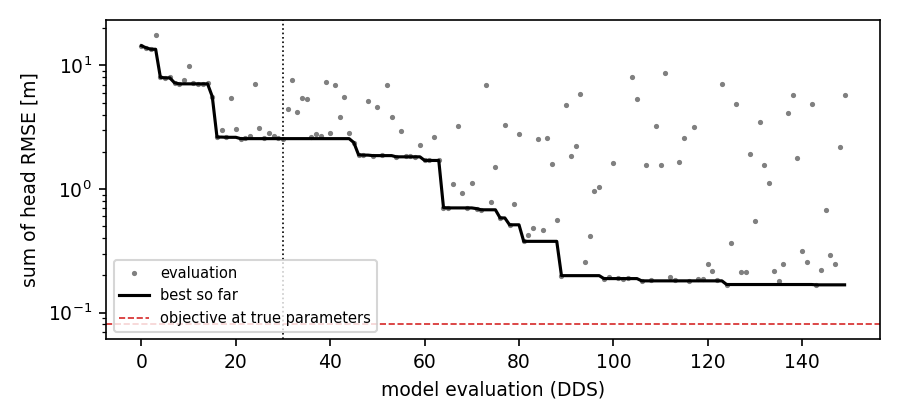
\includegraphics[width=0.8\linewidth]{figures/fig_calibration.png}
\caption{Synthetic calibration: objective against model runs.}\label{fig:calib}\end{figure}

\subsection{The Ostrich input file, line by line}
\begin{lstlisting}
ProgramType         DDS             # search algorithm (dynamically dimensioned search)
ObjectiveFunction   GCOP            # general constrained optimization
ModelExecutable     ./Ost-Raven.sh  # script that runs Raven in ./model
BeginFilePairs
  Liard.rvp.tpl ; model/Liard.rvp   # template -> model file with values filled in
EndFilePairs
BeginParams                         # name, start, lower, upper, transformations
  par_K_gravel   5.0  1.0  500.0  none log10 none
  par_Sy_gravel  0.10 0.05 0.35   none none  none
  par_K_till     2.0  0.01 5.0    none log10 none
EndParams
BeginResponseVars                   # values read from Diagnostics.csv
  RMSE1  model/output/Diagnostics.csv ; OST_NULL 1 4 ','  # line 1 (header = 0), column 4
  ...
EndResponseVars
BeginTiedRespVars                   # objective = sum of the RMSEs
  SUM_RMSE 4 RMSE1 RMSE2 RMSE3 RMSE4 wsum 1.0 1.0 1.0 1.0
EndTiedRespVars
BeginGCOP
  CostFunction SUM_RMSE
EndGCOP
BeginDDSAlg
  MaxIterations 150
EndDDSAlg
\end{lstlisting}
Ostrich counts the lines of \cmd{Diagnostics.csv} from 0 (the header is line 0) and its columns from 1. With
\cmd{:EvaluationMetrics NASH\_SUTCLIFFE RMSE KLING\_GUPTA} the columns are the series, the file, NSE, RMSE (column 4) and
KGE. The four \cmd{GW\_HEAD} series are lines 1--4 when they are the model's only observations. With four monitoring wells
added to the Liard example, whose 29 streamflow series come first, they are lines 30--33. Check the line and column of
each response in your own \cmd{Diagnostics.csv}: they depend on the order of observations and on
\cmd{:EvaluationMetrics}. To combine heads and streamflow, add NSE or KGE responses of the hydrographs with suitable
weights.
